\subsection{Gazebo Closed-Loop Validation in a Dense Urban Environment}
\label{sec:gazebocity}
We integrate the learned planner with the \texttt{suav1} flight model in Gazebo 11 and ROS Noetic to evaluate online execution in an urban scene. The environment combines existing building meshes with eight additional towers of 90--125 m height. The planning map contains 162 axis-aligned collision boxes, each expanded by 2 m at its faces. The aircraft starts at $(-90,-270,40)$ m heading north and follows eight waypoints with target altitudes of 40--60 m, including three waypoints through the city interior. Waypoint acceptance thresholds are 48.825 m horizontally and 3 m vertically.

The deployment planner runs at 10 Hz with $H=3$ s, $B=6$ s and $K=12$, using the frozen learned weights and feasibility-only ranking. It augments the seven coarse altitude targets with state-relative levels for gradual climbing and descending, giving up to 406 primary controls. The preceding comparative experiments retain their frozen 203-control library. The Gazebo plugin integrates point-mass flight dynamics and first-order actuator responses at a 0.004 s simulation step, then updates the aircraft velocity and attitude. Initial airspeed is 13.5 m/s, and the commanded cruise speed is 15.5 m/s.

A body-mounted three-dimensional lidar provides 512 horizontal samples across 360$^\circ$ and 32 vertical lines spanning $-40^\circ$ to $20^\circ$, at 5 Hz with a 1--120 m range. Ray intersections with Gazebo collision geometry generate the returns. The mapping node interpolates the simulation odometry at each scan time and accumulates occupied endpoints on a 2 m voxel grid; RViz displays the current scan, map and flight trajectory. Planning uses the supplied building collision map, while the lidar map records the observed environment.

Figure~\ref{fig:gazebocity} presents the recorded flight and lidar map, and Table~\ref{tab:gazebocity} summarizes this run. The aircraft completes the eight-waypoint cycle at $t=90.408$ s. Each of the 902 logged planning updates selects a continuation-verified primary. The minimum aircraft-reference-point distance to the physical boxes is 11.563 m, and the corresponding minimum distance to the expanded boxes is 9.098 m. Recorded states remain outside both sets of boxes. The maximum absolute bank angle is 34.999$^\circ$, and the maximum absolute flight-path angle is 16.299$^\circ$, within their respective 35$^\circ$ and 20$^\circ$ limits. All eight added towers produce lidar returns. The final stored map contains 163,777 occupied cells without capacity eviction. This urban flight demonstrates online integration of learned continuation search, vehicle execution and lidar acquisition; the multi-map comparisons above quantify the scheduling performance.

\begin{figure*}[!t]
\centering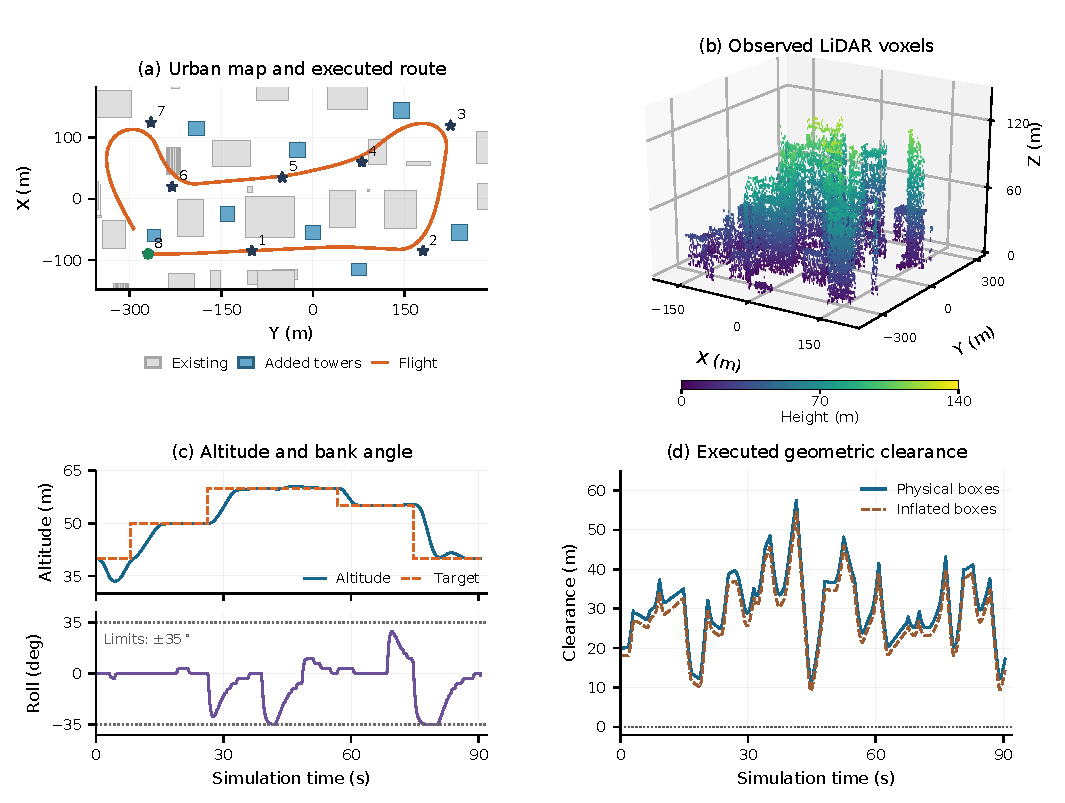
\includegraphics[width=.98\textwidth]{figures/gazebo_city.pdf}
\caption{Recorded Gazebo flight in the dense urban scene. (a) Building footprints and the executed trajectory, with $Y$ horizontal and $X$ vertical. Blue footprints identify the added towers, stars mark waypoints and the green dot marks the initial recorded position. (b) Occupied 2 m lidar voxels colored by height. The view omits cells at or below 2 m and displays every fourth remaining cell (17,822 of 71,286). (c) Recorded altitude and bank angle, with target altitude and bank limits. (d) Aircraft-reference-point clearance to the physical and expanded collision boxes. All panels are reconstructed from saved simulation data; the occupied map in (b) is obtained from lidar returns.}
\label{fig:gazebocity}
\end{figure*}

\begin{table}[!t]
\centering\small
\caption{Urban Gazebo run. Clearances refer to the aircraft reference point. Scan acquisition ends at 90.408 s; the last periodically published map is stamped 89.808 s.}
\label{tab:gazebocity}
\begin{tabular}{lr}
\toprule
Quantity & Recorded value \\
\midrule
Completed waypoints & 8 \\
Cycle completion time (s) & 90.408 \\
Logged / continuation-verified updates & 902 / 902 \\
Minimum physical-box clearance (m) & 11.563 \\
Minimum expanded-box clearance (m) & 9.098 \\
Maximum absolute bank angle ($^\circ$) & 34.999 \\
Maximum absolute flight-path angle ($^\circ$) & 16.299 \\
Received lidar scans & 452 \\
Occupied voxels in the last map & 163,777 \\
\bottomrule
\end{tabular}

\end{table}
